\section{问题三，单品选择与定价优化}

\subsection{候选单品池}

问题三要求从 6 月 24 日至 30 日实际有销售的单品里挑。从销售记录中提取这 7 天有交易的全部 $49$ 个单品，按品类统计如表 \ref{tab:q3_candidates}。

\begin{table}[H]
\centering
\caption{候选单品池概况（6 月 24 日至 30 日）}
\label{tab:q3_candidates}
\begin{tabular}{lcccc}
\hline
品类 & 候选单品数 & 占比 & 日均品类需求 (kg) & 约束状况 \\
\hline
花叶类 & 17 & 34.7\% & 124.8 & 宽裕 \\
辣椒类 & 10 & 20.4\% & 77.6 & 宽裕 \\
食用菌 & 8 & 16.3\% & 44.2 & 宽裕 \\
水生根茎类 & 7 & 14.3\% & 16.7 & 充裕 \\
茄类 & 5 & 10.2\% & 19.0 & 充裕 \\
花菜类 & $\mathbf{2}$ & $\mathbf{4.1\%}$ & 16.2 & \textbf{瓶颈} \\
\hline
\end{tabular}
\end{table}

花菜类只有 $\mathbf{2}$ 个单品这一周有交易。不管怎么优化，两个单品一定会被选中，不存在替代。如果后来发现其中某单品利润率为负，也没有其他花菜类单品可以顶上。这是本节模型的结构性约束，不是调参数能解决的。

\subsection{双层规划}

实际超市选品过程天然是两层的，品类经理拍板各品类占多少货架位，采购再在每个品类里挑具体单品。模型跟着这个结构走。

\subsubsection{上层，品类配额}

各品类最低 SKU 数按候选池占比比例分配，目标总数 $S=30$（区间 $[27,33]$ 中点），

\begin{equation}
k_i = \text{clip}\left( \text{round}\left( \frac{n_i}{\sum_j n_j} \times S \right), 1, n_i \right)
\end{equation}

花菜类候选只有 $2$ 个但按比例至少要有 $2$ 个，所以 $k=2$，两个全取。分配结果，花叶类 $10$、辣椒类 $6$、食用菌 $5$、水生根茎类 $4$、茄类 $3$、花菜类 $2$。剩余 $\sum k_i - 30$ 个名额按评分从高到低补满。

\subsubsection{下层，单品评分与选品}

每个候选单品 $j$ 的综合评分用三项加权，

\begin{equation}
s_j = 0.5 \cdot \frac{m_j}{\max(m)} + 0.3 \cdot \frac{d_j}{\max(d)} + 0.2 \cdot \left(1 - \frac{r_j}{|C(j)|}\right)
\end{equation}

其中 $m_j$ 是单位利润（元/kg），$d_j$ 是日均销量（kg），$r_j/|C(j)|$ 是品类内销量排名分位。权重给利润最大（$0.5$），因为目标是收益最大化；其次看销量保证基本需求覆盖；排名分位是弱的多样性偏好，品类内排名靠后的单品不会因为评分稍低就被完全排除。

实际操作分两步，Phase 1 强制每品类取评分最高的 $k_i$ 个单品，Phase 2 把剩下名额按评分从高到低补满到 $30$ 个。

\subsubsection{单品最优定价}

入选单品独立优化加成率。需求函数复用 Q2 估计的品类级弹性 $\beta_{C(j)}$（这里用了品类弹性近似单品弹性，后面会专门讨论这个问题），

\begin{equation}
r_j^* = \arg\max_{r \in [0.05, 3.0]} \quad (P_j(r) - C_{\text{eff},j}) \cdot \max\left(d_{\text{base},j} \cdot \left(\frac{P_j}{P_{\text{hist},j}}\right)^{\beta_{C(j)}}, 2.5\right)
\end{equation}

定价、补货量与选品三者在这个框架下同时求解，不是先选品再单独定价。

\subsection{优化结果}

\begin{table}[H]
\centering
\caption{Q3 单品选品与定价结果（7 月 1 日）}
\label{tab:q3_results}
\begin{tabular}{lcccc}
\hline
品类 & 入选单品数 & 补货量 (kg) & 预期利润 (元) \\
\hline
花叶类 & 10 & 60.4 & 391.9 \\
辣椒类 & 6 & 34.9 & 243.6 \\
水生根茎类 & 4 & 10.9 & 190.7 \\
花菜类 & 2 & 11.8 & 171.0 \\
食用菌 & 5 & 15.9 & 126.3 \\
茄类 & 3 & 13.4 & 101.8 \\
\hline
合计 & $\mathbf{30}$ & $\mathbf{147.2}$ & $\mathbf{2,060.4}$ \\
\hline
\end{tabular}
\end{table}

三项约束全部满足，30 个单品在 $[27,33]$ 区间内；各单品订货量 $\geq 2.5$ kg；每个品类至少有一个代表作；花菜类的 2 个候选单品都入选了。单日预期收益 $\mathbf{2,060}$ 元。

和基线（M2，贪心选品加固定加成率 $20\%$）的对比值得单独说。M2 也是 30 个单品，但单日利润只有 $253$ 元，差了将近 $\mathbf{5}$ 倍。差距几乎全部来自加成率，M2 里所有单品统一按成本 $+20\%$ 定价，而 M1 的内生优化在数据支持下给出了远更高的加成水平。这一差距反过来验证了 Q2 弹性估计的结论，在现有数据覆盖的价格区间内，蔬菜需求的价格弹性可能被传统 $20\%$ 加成率的经验规则低估了。

\subsection{本节关键局限}

\textbf{单品弹性借用品类弹性}。这是本节最根本的方法论局限。Q2 的弹性是对一个品类里所有单品的平均估计，Q3 直接把它套在每个单品头上。品类内不同单品的价格敏感度可能有巨大差异，云南生菜（明星单品）比某个小众绿叶菜的弹性低得多，用同一个 $\beta$ 会抹平这种差异。结果就是所有单品的加成率都冲向同一个方向。

\textbf{花菜类的系统性脆弱}。只有 2 个候选单品意味着该品类的供应韧性为零。任何一个单品断供或者质量出问题，花菜类就从当天货架上消失。

\textbf{单日优化 vs 多日规划}。本模型只优化 7 月 1 日一天。如果放宽到 7 天联合决策，可能会在不同天选不同的单品组合，比如辣椒类的某个品种只在周三销量高，总利润比单日最优的简单加总更高。但题目限定了"根据 6 月 24 日至 30 日的可售品种给出 7 月 1 日的决策"，所以没有往后多算。

\begin{figure}[H]
\centering
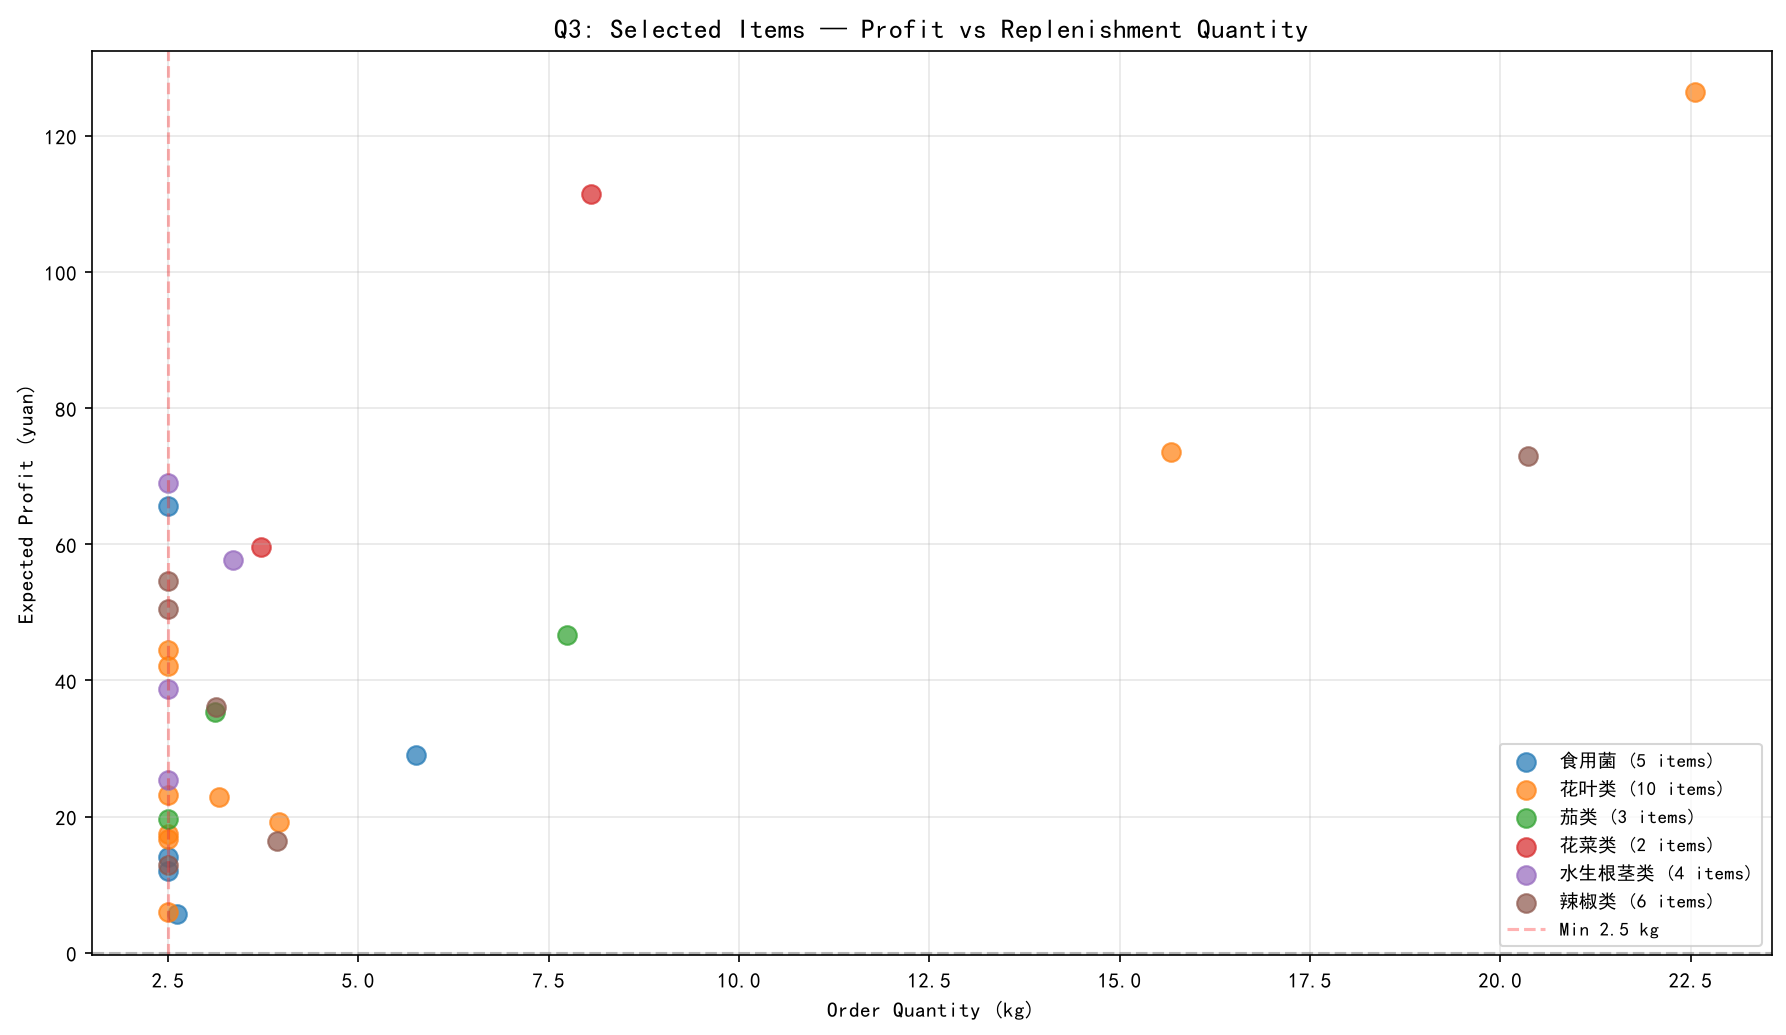
\includegraphics[width=0.85\textwidth]{paper/figures/fig_q3_scatter.png}
\caption{30 个入选单品利润与补货量散点图（按品类着色），最小陈列量线标为红色虚线}
\label{fig:q3_scatter}
\end{figure}

\begin{figure}[H]
\centering
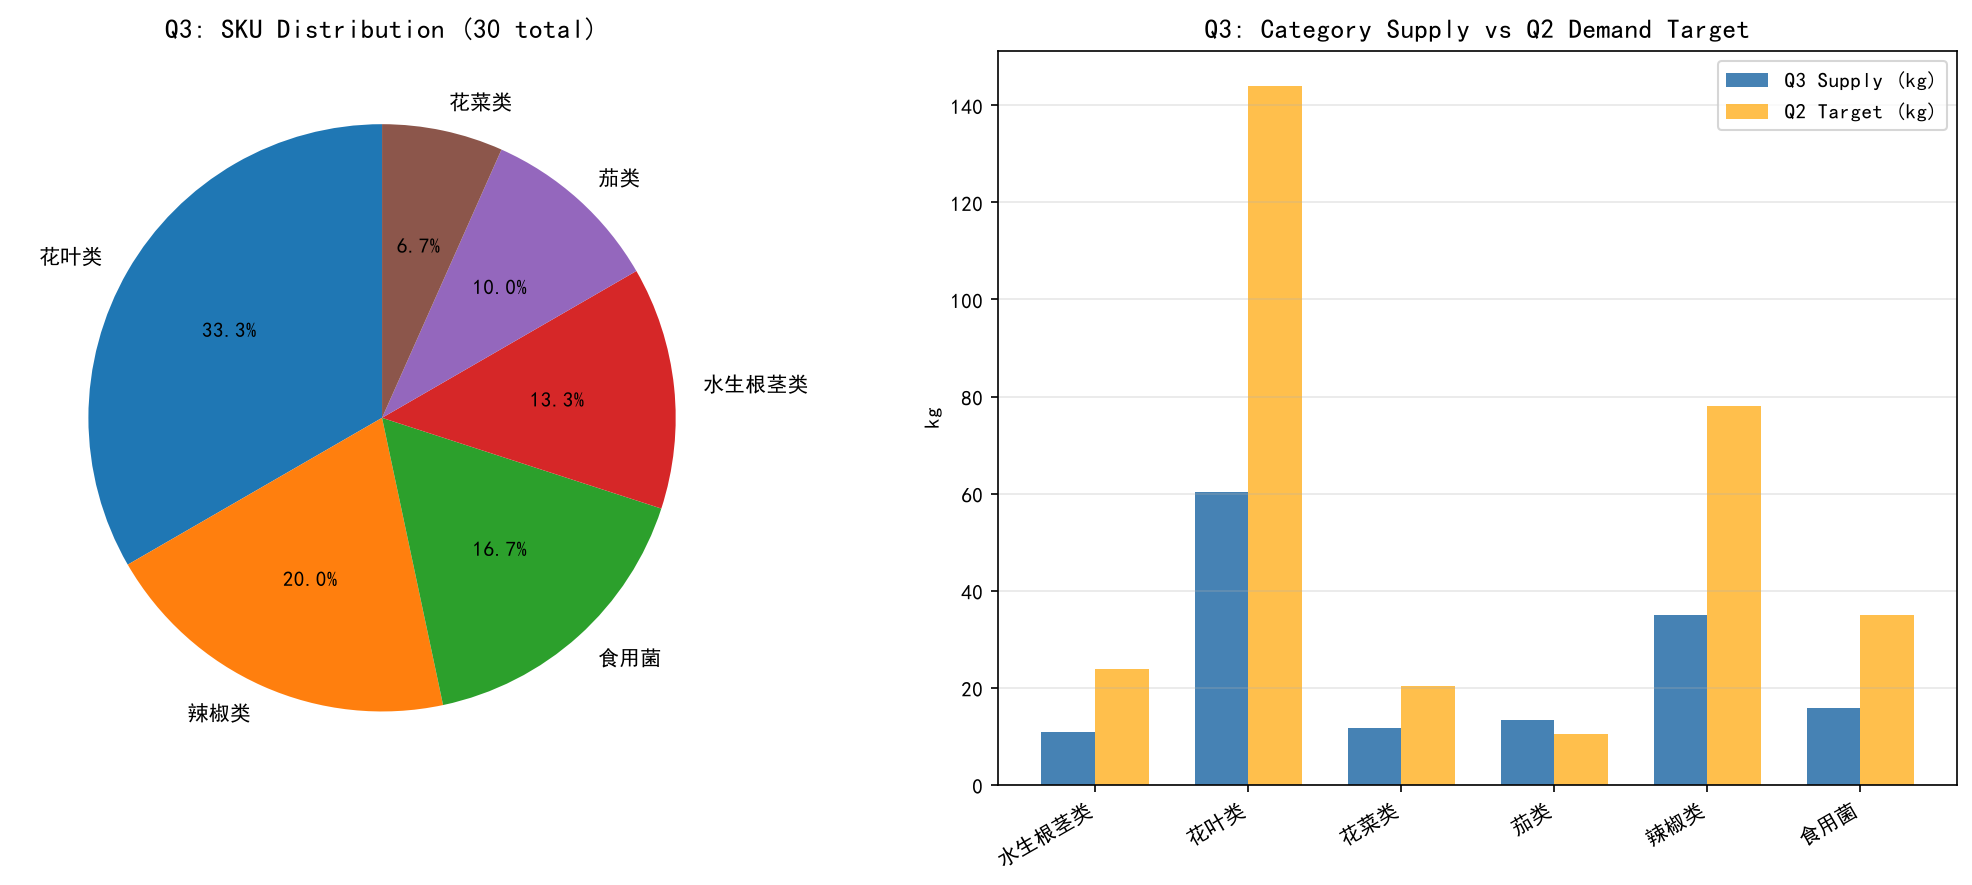
\includegraphics[width=0.85\textwidth]{paper/figures/fig_q3_fulfillment.png}
\caption{各品类补货量 vs 问题二品类需求目标}
\label{fig:q3_fulfillment}
\end{figure}
